\documentclass[MachineLearning]{subfiles}
\begin{document}

%@@@@@@@@@@@@@@@@@@@@@@@@@@@@@@
% summarizes lecture 4 and tutorial 3
% author: Benjamin Ellenberger

\section{Numerical Estimation Techniques}
The main problem of estimators is that we would like to be able to compute the expectation of some statistic such as the prediction error: \[\printlatex{ \predR(c) = \E[\overbrace{\I_{\{c(x) \neq y\}}}^{\hidewidth\text{Indicator function counts errors}\hidewidth}] =  \sum^k_{y=1}\int\I_{c(x_i)\neq y_i}P(x,y)dx}\] But we can only estimate the empirical mean \[\printlatex{\hat{\predR}(c) = \frac{1}{n} \sum_{i\leq n}\I_{c(x_i)\neq y_i}}\] from the data we have.\\
The question is how far is \(\printlatex{\predR(c)}\) from \(\printlatex{\hat\predR(c)}\) and how different are the prediction functions \(\printlatex{c^{opt} \in \argmin_{c(x)} \predR(c)}\) and \(\printlatex{\hat c(x) \in \argmin_{c(x)} \hat\predR(c)}\)?


\subsection{Cross-Validation}
Cross-validation is a model validation technique for assessing how the results of a statistical analysis (here a prediction) will generalize to an independent data set. In a prediction problem, a model is usually given a dataset of known data on which training is run (\textbf{training dataset}), and a dataset of unknown data (or first seen data) against which the model is tested (\textbf{testing dataset}). The goal of cross validation is to define a dataset to "test" the model in the training phase (\textbf{validation dataset}), in order to limit problems like overfitting, give an insight on how the model will generalize to an independent data set. (Wikipedia)


\subsubsection{K-fold Cross validation}
In K-fold cross-validation, the original data is randomly partitioned into K equal size subsets.
\begin{figure}[H]
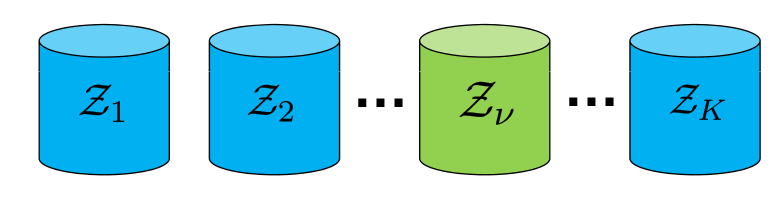
\includegraphics[width=0.8\linewidth]{figs/cross-validation-subsets}
\end{figure}
Of the K subsets, a single subset \(\printlatex{\mathcal{Z}_v}\) is retained as the validation data for testing the model, and the remaining \(\printlatex{K - 1}\) subsets are used as training data with \(\printlatex{n \frac{K-1}{K}}\) data samples.

\begin{figure}[H]
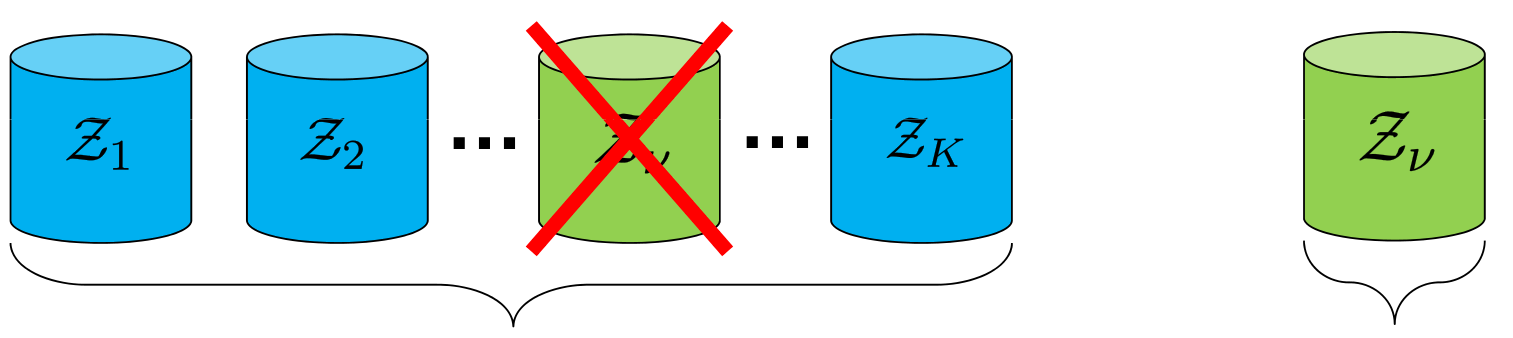
\includegraphics[width=0.8\linewidth]{figs/cross-validation-testing-validation-set}\\
Data sets:\hspace{4em}Training data set to learn \(\printlatex{\hat c^{-\mathcal{Z}_v}(x)}\)\hspace{6em}Validation data
\end{figure}

 The cross-validation process is then repeated K times (K-fold), with each of the K subsets used exactly once as the validation data. The K results from the folds can then be averaged (or otherwise combined) to produce a single estimation. \[\printlatex{\hat\predR^{cv} = \frac{1}{K} \sum_{v \leq K} \hat\predR_v = \frac{1}{n} \sum_{i\leq n} \I_{\{y_i\neq \hat c^{-\mathcal{Z}_{v(i)}}(x_i)\}}}\]
\(\printlatex{\hat c^{-\mathcal{Z}_{v(i)}}(x_i)}\) is the classifier which has been trained by omitting the data \(\printlatex{(x_i,y_i) \in \mathcal{Z}_{v(i)}}\). The \(\printlatex{\mathcal{Z}_{v(i)}}\) is then used for the error estimation.


\subsubsection{Leave one out method}
When \(\printlatex{K=n}\) (the number of observations), the K-fold cross-validation is exactly the leave-one-out cross-validation.\\


\subsubsection{Engineer's solution to bias-variance problems}
\textbf{Problem:} Highly correlated training sets can cause large prediction error variantion.\\
\textbf{Solution:} Choose K in K-fold cross validation as \(\printlatex{min\{\sqrt{n},10\}}\).


\subsubsection{Cross-validation guided Model selection}
Adapt feature set by subset selection and control it by minimizing the prediction error. Note that it is important to calculate the final prediction error on data
which have not been used in model fitting (training) nor in model selection (testing for parameter adaptation). Therefore you can split your data set again into more subsets for this.

\begin{enumerate}
\item Run cross-validation for every value of the hyperparameter \(\printlatex{(\lambda,\mathcal{C},\ldots)}\)
\item Choose the value corresponding to the lowerst prediction error.
\item However you can not report this error as the generalization error of your algorithm, as the algorithm has seen all the data for model selection when choosing your hyperparameter.
\item So you need a separate dataset to evaluate the generalization error.
\end{enumerate}


\subsection{Bootstrapping}
Bootstrapping is the practice of estimating properties of an estimator (such as its variance, bias, variance, confidence intervals, prediction error or some other such measure) by measuring those properties when sampling from an approximating distribution. One standard choice for an approximating distribution is the empirical distribution of the observed data. In the case where a set of observations can be assumed to be from an independent and identically distributed population, this can be implemented by constructing a number of resamples with replacement, of the observed dataset (and of equal size to the observed dataset). (Wikipedia)

\begin{figure}[H]
\centering
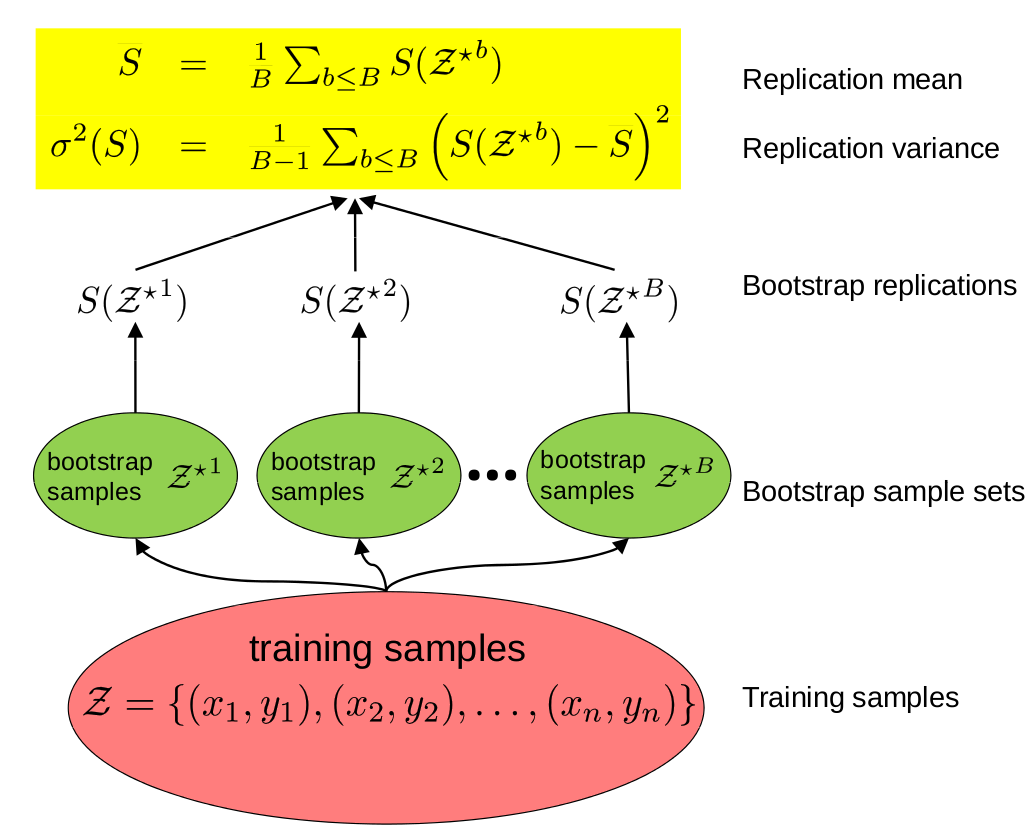
\includegraphics[width=0.8\linewidth]{figs/bootstrapping-process}
\end{figure}

\paragraph{Goal of Bootstrap}
Calculate numerically the estimation error of a statistic S(Z), e.g., the probability of error \(\printlatex{\hat\predR(\hat c(x))}\) for classifier \(\printlatex{\hat c(x)}\) based on the empirical distribution function \(\printlatex{\hat F_X(x)}\). We approximate \(\printlatex{F_X}\) by the empricial data source \(\printlatex{\hat F_X}\)\\
Consistency of the bootstrap estimate:\\
\[\printlatex{\lim\limits_{B \rightarrow \infty}\frac{1}{B - 1} \sum _{b \leq B} \left(S(\mathcal{Z}^{*b})-\frac{1}{B} \sum_{\beta \leq B} S(\mathcal{Z}^{*\beta})\right)^2 = \V_{\hat F}[S(\mathcal{Z})]}\]
Bootstrap works if the deviation between empirical and bootstrap estimator
( \(\printlatex{\hat F}\) being the Bootstrap CDF) converges in probability to the
deviation between true parameter value and the empirical
estimator, i.e. \(\printlatex{\predR^{str}_n ( \hat F, \hat F^* ) - \predR^{str}_n (F, \hat F) \overset{P}{\rightarrow} 0,\text{for }n\rightarrow \infty}\) where \(\printlatex{\predR^{str}_n}\) is one of the following:
\begin{itemize}
\item Error distribution: \(\printlatex{\predR^{err}_n (F,\hat F) = P(\sqrt{n}(S(\hat F) - S(F)))}\)
\item Bias: \(\printlatex{\predR^{bias}_n (F,\hat F) = \E_F[S(\hat F)] - S(F)}\)
\item Standard error: \(\printlatex{\predR^{std}_n (F,\hat F) = \sqrt{\E_F[(S(\hat F) - S(F))^2]}}\)
\end{itemize}
\todo[inline]{ Describe the \(e_0\) bootstrap estimator if that is needed.}


\subsection{The "Jackknife" Method}
In statistics, the jackknife is a resampling technique especially useful for variance and bias estimation. The jackknife predates other common resampling methods such as the bootstrap. The jackknife estimator of a parameter is found by systematically leaving out each observation from a dataset and calculating the estimate and then finding the average of these calculations. Given a sample of size \(\printlatex{N}\), the jackknife estimate is found by aggregating the estimates of each \(\printlatex{N-1}\) estimate in the sample. (Wikipedia)


\subsubsection{Estimation}
The jackknife estimate of a parameter can be found by estimating the parameter for each subsample omitting the ith observation to obtain an estimate \(\printlatex{\bar{\theta}_i}\). The overall jackknife estimator is found by averaging each of these subsample estimators.

\[\printlatex{\bar{\theta}_\mathrm{Jack} =\frac{1}{n} \sum_{i=1}^n (\bar{\theta}_i)}\]


\subsubsection{Bias estimation and correction}
The jackknife technique can be used to estimate the bias of an estimator calculated over the entire sample.

\[\printlatex{\bar{\theta}_\mathrm{BiasCorrected} = N \bar{\theta}-(N-1) \bar{\theta}_\mathrm{Jack}}\]
This reduces bias by an order of magnitude, from \(\printlatex{O(N^{-1})}\) to \(\printlatex{O(N^{-2})}\).

This provides an estimated correction of bias due to the estimation method. The jackknife does not correct for a biased sample. Bias corrected estimators can have a considerably larger variance than uncorrected estimators!


\subsubsection{Variance estimation}
An estimate of the variance of an estimator can be calculated using the jackknife technique.

\[\printlatex{\V(\theta) = \V(\frac{\sum_{i=1}^n (X_i)}{n}) = \frac{\sigma^2}{n} =\frac{n-1}{n} \sum_{i=1}^n (\bar{\theta}_i - \bar{\theta}_\mathrm{Jack})^2}\]
where \(\printlatex{\bar{\theta}_i}\) is the parameter estimate based on leaving out the ith observation, and \(\printlatex{\bar{\theta}_\mathrm{Jack}}\) is the jackknife estimator based on all of the samples.
\todo[inline]{Improve the text on the jackknife to fit the quality of the content of the lecture (Expansion not understood by Benjamin)}


\subsection{Hypothesis Testing}
\begin{enumerate}
\item Define the null hypothesis \(\printlatex{\mathcal{H}_0}\) (devil’s advocate).
\item Define the alternative \(\printlatex{\mathcal{H}_1}\) (one sided/two sided).
\item Find the test statistic.
\item Decide on the type I error \(\printlatex{\alpha}\) that you are willing to take.
\item Compute the Probability of observing the data given the null hypothesis: P-value.
\item Compare the P-value to \(\printlatex{\alpha}\); if it is smaller, reject \(\printlatex{\mathcal{H}_0}\).
\item We define a \textbf{Type I error} as the test accepts \(\printlatex{\mathcal{H}_0}\) if in reality it is false (false negative).
\item We define a \textbf{Type II error} as the test rejects \(\printlatex{\mathcal{H}_0}\) if in reality it is true (false positive).
\end{enumerate}


\subsubsection{Neyman-Pearson Test}
Selects a decision rules which minimizes the Type I error and fixes the Type II error.
\todo[inline]{Describe the Neyman-Pearson Test. Not understood by Benjamin}

\subsection{Readings}
\begin{enumerate}
\item Duda 2ed
\end{enumerate}
\todo[inline]{Write down readings from the books covering the topics of the Numerical Estimation Techniques section.}

\end{document}